% This example An LaTeX document showing how to use the l3proj class to
% write your report. Use pdflatex and bibtex to process the file, creating 
% a PDF file as output (there is no need to use dvips when using pdflatex).

% Modified 

\documentclass{l3proj}

\usepackage[legalpaper, portrait, margin=1.2in]{geometry}
\usepackage[utf8]{inputenc}
\usepackage{tabu}
\setlength{\parindent}{0pt}
\setlength{\parskip}{6 pt}

\usepackage{graphicx}
\graphicspath{ {images/} }

\begin{document}


\title{Building Healthy Communities Database}

\author{David Robertson \\
Maria Papadopoulou \\
David Andrew Brown \\
Kiril Ivov Mihaylov \\
Christopher Sean Harris \\
Jaklin Yordanova}

\date{\today}

\maketitle

\begin{abstract}

Building Healthy Communities in Dumfries and Galloway is a community development programme which aims to advance the health and well-being of all individuals within its area, but particularly those in difficult circumstances. Its main goal is to improve the lives of people who may otherwise become isolated, by encouraging participation in initiatives which help keep them physically and mentally healthy while also promoting the creation and sustaining of social bonds. The programme consists of three different types of participants:
\begin{itemize}
	\item Administrators
	\item Volunteers
	\item Members
\end{itemize}
Members are the individuals participating in the initiatives themselves. Volunteers run the initiatives and are responsible for tracking the members progress. They must inform administrators not only about the progress of the members but also about the whole process. Currently all this is being performed by hand. Administrators must manually input the data into a database, and also search the database using only inbuilt functions of the database software. This is a difficult and time consuming process. 

Our team was responsible for building a system to automate the input and retrieval of relevant data. We designed and implemented a system that accepts the current database, and allows it to be modified and extended. The system has the following features:
\begin{itemize}
	\item Registering new members and deleting those who leave the program
	\item Keeping track of members' attendance
	\item Keeping track of the progress of both members and volunteers
	\item Deleting and adding initiatives
	\item Searching the database for particular parameters and organising the information in an easy to read manner.
\end{itemize} 

\end{abstract}

%% Comment out this line if you do not wish to give consent for your
%% work to be distributed in electronic format.
\educationalconsent

\newpage

%==============================================================================
\section{Introduction}

Software engineering 

Third year undergraduates on the Computing Science course of the University of Glasgow undergo a year long team project, the aim of which is to give the students experience of working in a team on an extended software engineering project. It helps to develop an ability to work with customers, and teaches the use of agile software development practices and methodologies. Importantly, it also teaches the value of retrospection; the act of looking back to see what can be improved in future. With this case study, our intention was to analyse and explore the methods and practices we employed, in order to hopefully better understand their intricacies, how they should be used in a project such as ours, and to potentially develop new, better ways of applying these methods in future.

This paper presents a case study of the building of a database system for the public health program "Building Healthy Communities", and the development practices we used in the process. The BHC system is designed to replace the cumbersome, manual database currently in use by the NHS team that administers the BHC initiatives. It is intended to be a much more streamlined service, allowing for much faster input and retrieval of data from the system, while also allowing for varying levels of access, depending on who is using the system. The aim of the BHC programme is to encourage individuals who may be experiencing difficulties to lead healthier, less isolated lives through a collection of healthy living initiatives, and a system which allows for the secure, rapid organisation of data helps to ensure this aim can be easily met.

Through the following pages we will explain in more depth how we designed, created and use the software that we have described above using not only our previous knowledge, but also the knowledge that we have managed to gain from the University's courses. More specifically, the "Professional Software Development and SIT" course and the "Interactive Systems 3" course played a critical role in every step that we took in creating the software. From the requirements gathering to the coding of the software, close study of the material allowed for the development process to be much smoother than would have otherwise been the case, and led to a more polished product.

%% Incomplete paragraph
%%A paragraph written in the end describing the structure of the paper

Our dissertation is being divided..

%==============================================================================
\section{Case Study Background}

\subsection{Customer Organisation and Background}
\label{customer}

Building Healthy Communities is an NHS programme based in Dumfries and Galloway, utilising the concept of 'Healthy Living Centres'. Founded in 2001, it is a partnership of public, community, and voluntary organisations that operates regionwide to improve the health, wellbeing and quality of life of all people, particularly those in difficult circumstances. The programme consists of a Regional Partnership of strategic and local representation to help shape and direct, and four local Area Partnerships operating across the region. These Area Partnerships co-ordinate and take collective action by creating intiatives to tackle community health issues and the root causes of ill health.

The primary method by which Building Healthy Communities tackles its main objective is the creation and running of health initiatives. These are regular events, run by community members, for community members, with the aim of bettering the leath of individuals and the community as a whole. They foster a sense of well-being, and focus on people who might not otherwise be engaged in social events and feel isolated. Individuals are given the opportunity to become Community Health Volunteers through training and one-to-one support. This allows members of the community to feel even more active and helpful in their community.

While initiative events are run by volunteers from the local communities, the programme itself is run and maintained by a group of NHS employed administrators. These administrators are NHS employees, and have access to all the data produced by the programme. This includes the personal and medical details of all service users and volunteers, along with their feedback forms, and the funding status of every initiative. For the duration of the project, we were in contact with two of these administrators. They attended each customer meeting, and were instrumental in the shaping of our product, providing requirements and feedback. We also had some incidental contact with another NHS employee from the same area running a different project, whose advice was of particular use when designing the database and deciding which informtaion needed to be included.

\subsection{Initial Objectives for the project}
\label{objectives}

The initial objectives for the project were to develop a software, which will be used from the members, volunteers and administrators of the programme. All of those different groups of users have different level of access to the Database. The members would use the software to  complete a small questionnaire and give a regular feedback for the initiatives they attend. Volunteers, on the other hand, would be able to view that feedback and check the attendance of the members for the initiative they are assigned to. Administrators have the access and rights to do everything : they can see all the information about both volunteers and members, the can add or delete an initiative and review feedback and attendance as well. Since we are working in a Agile Team Organisation, the initial requirements could be slightly changed in the following customer meetings as explained later in the dissertation.

%==============================================================================
\section{Agile programming and Team organisation}

\subsection{Team organisation}
\label{organisation}

In our initial meetings, every team member pointed out their strong and weak parts in order to divide the work. Due to the fact that we were required to create an application and database from scratch, the workload was huge. As a result of that, everyone had to work in the "backend". Inevitable was for specific team members who were in a higher "backend/coding" level to execute some more advanced parts of the coding.
The team discussed various means of communication - we decided to avoid using common social media sites and to use the "slack" application, which provides a more organised and professional chat room with different channels. 

\subsection{Agile Methods}
\label{agile}

In terms of project planning, agile methods are one of the most trusted methods to use. Particularly, they are suitable for small teams and they involve frequent customer meetings because the requirements cannot be fully collected at the beginning of the software development cycle. Also, they are based on focusing on the code instead of the design which is suitable for our situation, since we were asked to develop a page from scratch requiring a database. Our project is based on one of the agile methods called "Extreme programming". This was the most suitable decision, due to the fact that we are novice programmers. One of the most useful features that Extreme Programming offers is called "pair programming" , which is highly occureing in our practices. As students, we lack of experience but when one student combine their knowledge with another, they can create spectacular results. Furthermore, user stories and prototyping helped us a lot to understand what really our application needed. Another important feature of Extreme Programming is the automated testing because as stated before, we have little experience.

\subsection{Technologies Used}
\label{tech}

As soon as we agreed on the methods we were going to use, we had to decide the technologies that we needed to use regarding project management. The university moodle page, suggested a series of technologies to use for handling our project such as "Ant and Ivy", "Jenkins", "Apache" etc. After a small group meeting and a discussion with the supervisors about what we are allowed to use and what we are not, we decided to use Gitlab for our project management and repository. Gitlab provides every technology that is needed to handle our project repository, the permissions that each member has as well as an amazing GUI that organises the "wiki" page and the "issues" page and so on. Using Gitlab, was very helpful, since we had all our due dates clearly displayed, issues and requests organised as milestones with the appropriate labels. The most useful feature that Gitlab provided to us was the Continuous Integration (CI) feature. CI is a tool that enables all the repository users to merge their work to a local repository. This was a huge organisational feature, since everyone could interact in the project code. Every team member, could assign a ticket to themselves or even to other team members, as a result we had a highly organised page where we could track the workload that every member has done. This was very helpful, in terms of assigning work to members that have not contribute as much as the others in a specific week and assign less to members that already have done more work than needed. Subsequently, we were making our issues very descriptive; using checkboxes, weight, time estimating and different labels. This was very useful in terms of tracking progress. A feature that contributed to the increment of the security of the software was the creation of a seperate branch for resolving any opened issues. Every particular issue or every new alternative was related with a newly created branch. In that way we were testing new features and bug fixes without pushing to the Master branch. Only after the problem was solved, a Merge Request was created followed by closing that particular issue and deleting the temporary branch. Lastly, a feature that the lead developers managed to add in subsequent time was the "Docker". Docker is an open source container platform. Docker can be described as the platform that worked for us. It offers an automated deployment of the software. The most important thing that Docker offers is that the deployments happens in different "containers" which hold all the requirements the software has. This results to a more automated management of the software.

 After this discussion, the meeting was not over. Therefore, we needed to decide which technologies would be used for implementing the project itself. We had to choose which web application framework to use. The first option we discussed was Django, due to the fact that every team member had previous experience with Django from our second year web application development course. Another option a team member suggested was Rails as more powerful tool with better documentation. To put more depth in it, Rails is a web application framework with "model-view-controller" software design pattern, not "model-view-template" like Django, which we were familiar with. None of the six members in our team coded on Rails before, so we have postponed our meeting and created an issue in the Gitlab - every member in the team had to study Rails in their time. In the next meeting, we voted and agreed to use Rails. Rails provides a massive help in the testing process. Moreover, the biggest factor that persuaded the team to work with Rails was the automation of many tasks and the "Gems" documentation that provides. "RubyGems" is a package manager. Using a tool called "Gem" in your terminal you can install and work with different libraries. Gems, are previously tested libraries, which provided security and saved a lot of valuable time. Reusing previously tested tools is always highly suggested in the world of web application frameworks.
  Since Rails, as previously stated, is based in "model-view-controller" we needed to find a model, an application to manage our newly created database. PostgreSQL was our choice because the database would be small with just a couple of thousand text records. Furthermore, PostgreSQL is a self-contained, free to use object-relational database management system.
 
 \subsection{Retrospective}
\label{retrospective}
 
 All these process, should be summarised in a page. Here is when we decided to use retrospectives. Retrospectives are a small summary of a past situation. In our course, retrospective is used to summarise our actions which were performed in a specific amount of time for progressing our project. Our retrospectives were created in "Trello". This was very helpful because we stated what we did good, what we were lacked of in knowledge and what we could improve. To be more specific, we decided to use 4L's: Liked, Lacked, Learned, Longed for. We also decided to create and fill a new retrospective every time we had a customer's meeting, which was the end of every Milestone and iteration as well.  Every team member was participating in the retrospective and filling at least one thing on the board. The team was raising an issue in the gitlab where when every team member was completing his/her retrospective was ticking their name. Additionally, an hour gap was allowed until the team meeting were each one individually would outline their thoughts and suggestion about the previous iteration. After that, the team was performing an hour long meeting which was followed by a discussion and outlining major issues that were identified through Trello. The team leader was navigating the meeting and organising a synopsis of all the team member's opinions in a paragraph. This was the most efficient way of observing problems and solving them as a team. Retrospectives helped to underline a major percentage of our issues in gitlab. Furthermore, we not only had time to improve, but also to learn new technologies and discover in more depth the needed technologies for accomplishing our tasks due for the next meeting.

\subsection{Team roles}
\label{roles}

Due to the fact that the team was composed from novice programmers, the team roles were not clearly defined by the first month. During the following month and after the first iteration the team had a meeting were the roles were clarified as follows:

\begin{itemize}

\item David Brown - Lead Developer, Docker Magician

\item David Robertson - Lead Developer

\item Chris Harris - Documentation

\item Kiril Mihaylov - Documentation and Front End Developer

\item Maria Papadopoulou - Documentation and Front End Developer

\item Jaklin Yordanova - Documentation and Front End Developer

\end{itemize}
 
The team voted about the actual team leader. The team leader will navigate any retrospective and any presentation of the application to the customers. Additionally, the team is following a role based model. Thus, the team leader is actually just a team manager, he is not taking the final decisions alone but with the team's help. The team leader is just helping to the navigation of the program and explaining the daily tasks. The team voted fairly David Brown as the team leader since he is the one of the back end lead developers and had the most contribution to the project. Applying roles, does not necessarily mean that any team member will not work in any other sectors of the website. The members faced many difficulties in resolving issues of the program, such that many times a work has been transferred to another member of the team. Furthermore, the workload of the back end development is massive and many minor issues were assigned to other team members than the "Lead Developers" so that the lead developers can focus in more advanced issues. Subsequently, we discovered the benefits from working in pairs for different tasks regarding the Documentation, researching and doing 'Pair Programming'. This was not only useful for our team building but also time-saving and code-efficient. 


%==============================================================================
\section{Documentation}
\label{documentation}

To begin with, we have divided our project to **number** different milestones which lasted a period between every customer meeting. In the following lines I will discuss the process that was taken in every milestone.

\subsection{Objectives}
\label{objectives} 

On the first customer meeting, the day that we were assigned our project, the customers underlined their desired program which I have stated above. By the end of the meeting, we asked the customers what the wanted to see in the next meeting, their answer was: "I guess, some sketches !". A new milestone was created with our next goal to be some basic documentation and the creation of some wireframes.

\subsection{Requirements Gathering}
\label{requirements}

During the meeting, we have managed to outline some basic requirements. We have had developed a wiki page containing an outline of the meeting. We have used this page to identify the functional and non-functional requirements. Having an on-going contact with the customers, who stated some useful points we ended up with the final version of the functional and non-functional requirements. 

The final version of the functional requirements is:
\begin{itemize}

\item An administrator should be able to view all information stored in the database.

\item An administrator should be able to add/remove/modify volunteers, members and groups that are stored in the database.

\item An administrator should be able to search and sort on specific fields belonging to tuples.

\item An administrator should be able to view data metrics on how particular groups/initiatives are progressing.

\item Different groups of users should have differing levels of permission to the data stored.

\item Volunteers should be able to view the data associated with their specific group(s), that they are allowed to see, and no other groups.

\item Volunteers should be able to record member attendance.

\item Provide a facility to register attendance.

\item Provide a facility to gather feedback from end users (members).

\end{itemize}

The final version of the non-functional requirements is:

\begin{itemize}

\item The system should be secure.

\item The system has to conform to the Data Protection Act.

\item The system should be stable whilst in use and have a high up time.

\item The system should be able to operate for long periods of time without intervention from system admins.

\item The system should be simple to use.

\item The system should be modular and hence maintainable.

\item The system should be lightweight.

\item The site should be compatible with many platforms. (Portable.)

\end{itemize}

Identifying the requirements was an important step which enabled us to put in action some examples. The team got divided into groups and documented various things such us user stories, user scenarios and wireframes. 

\subsection{User Stories}
\label{user_stories}

User stories play a critical role in the agile methods that we have chosen to follow. A user story formally describes the state of the application. The basic functions that a potential user expects it to do. We have managed to identify functional and non-functional user stories. User stories helped us to put in action the program and to fully understand how it will work.

A couple of highly representative functional user stories are:
\begin{itemize}

\item As an administrator, I want to add a member to the database, so that they can join a group.

	\begin{enumerate}
  	\item Add an activity to add a person
  	
	\item Add an activity to enter their information

	\item Add an activity for choosing groups

	\item Create a query for retrieving groups
	\end{enumerate}
\item As a volunteer, I want to be able to register attendance at my group(s), so that I can contribute data.

	\begin{enumerate}
	\item Create a query to retrieve groups I run
	
	\item Add an activity to log attendance
	
	\item Create a query for members of the group
	
	\item Add an activity to enter attendance per member
	
	\end{enumerate}

\item As a member, I want to be able to log in, so that I can view my information.

	\begin{enumerate}
	
	\item Add an activity to log in
	\item Add an activity to enter log in information
	
	\end{enumerate}

\end{itemize}

Thus, we had to record some non-functional user stories so that we can give practical examples about how the system will work. Some non-functional user stories are:

\begin{itemize}

\item  As an administrator, I want to replace a member's name with numbers in the database, so that I can find them easier.

	\begin{enumerate}
	
	\item Create a query for retrieving a person
	
	\item Add an activity to update a person's information
	
	\item Create a warning message for wrong type of input
	
	\item Do not allow this modifications to be saved
	\end{enumerate}
	
\item As a volunteer, I want to be able to have access to the database, so that I can add a new program that the administrators haven’t added yet.

	\begin{enumerate}
	\item Restrict the "Add a new page", "Add a new page", "Add a new member", etc buttons to can be only accessed from administrators
	\end{enumerate}
	
\item As a member, I want to be able to add or delete a group that I am part to, so that I can register my self to new groups or delete me from the old ones.

	\begin{enumerate}
	\item Restrict the member's redirected page to do very basic tasks
	\item Do not provide this functionality to members.
	\end{enumerate}

\end{itemize}

\subsection{User Scenarios}
\label{user_scenarios}

Although user stories provide a clear outline about what the users and system needs, there is nothing textual more representative than a scenario where an everyday user of the system will describe what they actually needs Thus, a couple of team members wrote some representative scenarios of example users. 
Example scenarios can be find bellow:
\begin{itemize}
\item Carolyn is an administrator in the Building Healthy Communities program. She is in charge of tracking the volunteers progress and checking if they are doing their work correctly. It is important for the program to not only track members attendance and feedback but also to track volunteers one. This is vital for keeping the program works correctly and also would be an advantage in building the relationship between members and volunteers.

\item Rebecca is a volunteer in the Building Healthy Communities program at the Arts group. She is currently working with a group of eight people. In the end of every session she collects attendance and feedback forms from the members. The process of reading and analyzing them is very time consuming. Various handwritten forms are messy and some information are not that useful. She would prefer to have an automatic program that does all this so she can completely skip the time she spends on tracking attendance and focus on improving the Art class based on the feedback provided.

\end{itemize}

\subsection{Wireframes}
\label{wireframes}

After collecting all this useful information, the team was ready to start developing some wireframes. Wireframes were the final goal of this milestone. Without completing them would be like we have not worked at all. Having a small research during the meeting, we decided to use balsamiq for the creation of the wireframes. Balsamiq is a very useful application, easy to use and focus on the creation of the wireframes. Before we started sketching in the balsamiq, the team decided to go pen and paper to sketch our ideas. Pen and paper sketches are always the best plan, they give you the freedom to design exactly what you need. 

The formal wireframes were ready for the presentation. A screenshot of the index page can be found in Figure 1.

\begin{figure}
  \centerline{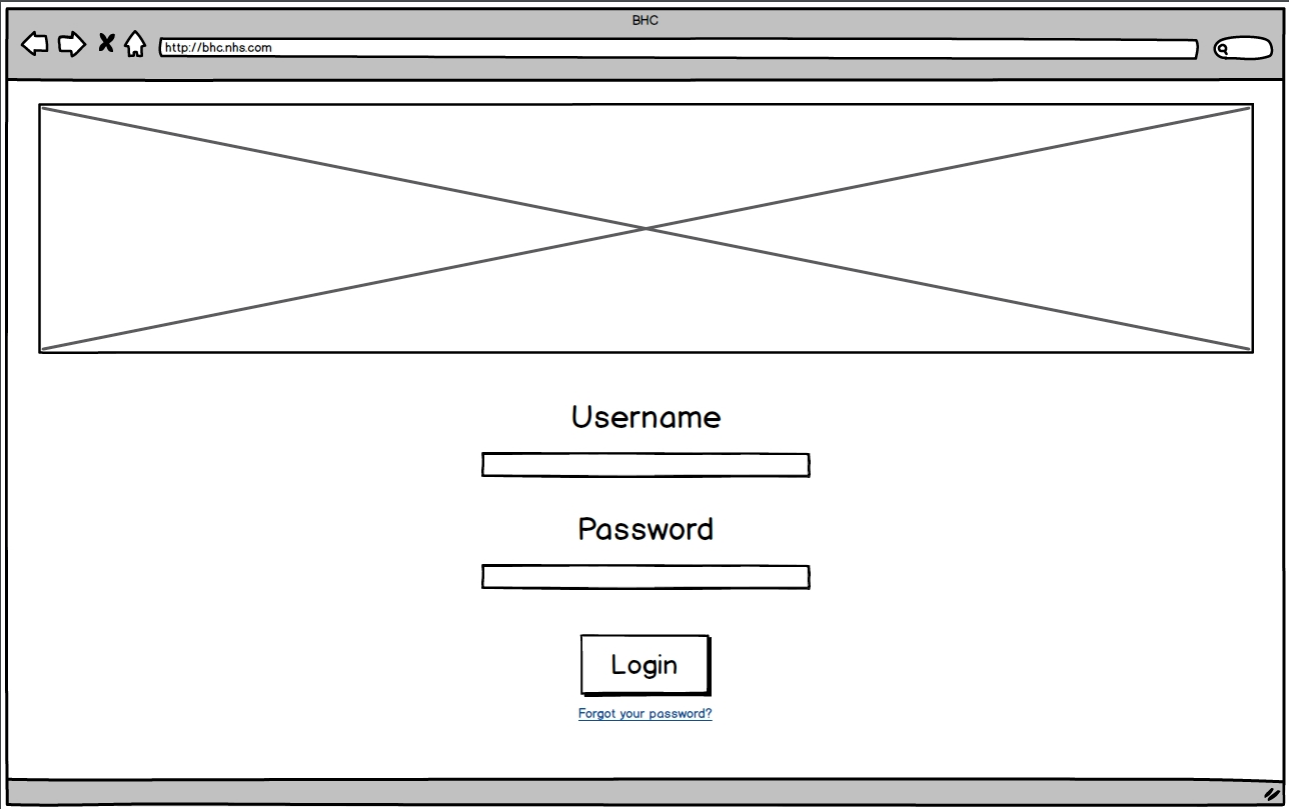
\includegraphics[width=\textwidth, height=\textheight, keepaspectratio]{wireframe.png}}
  \caption{Given structure of WireFrame}
  \label{fig:initialWireframe}
\end{figure}



\subsection{End of first milestone}
\label{sec:milestone1}

The second customer meeting was held on the 16th November. In the meeting we have outlined some examples of user scenarios and a brief tour through our interactive wireframes. An amount of time was available for the customers in order to express their opinion about our current progress and what do they expect from the team to be done until the next meeting.

An overall satisfaction was kept from both the team and the customers. After the meeting, the team filled a retrospective. An outline of the retrospective was that the team during this period of time improved its knowledge on using an application such us "Gitlab" as a project management tool. Moreover, we learned that in order to complete the project successfully, we need not only coding skills but strongly organisational skills with the huge amount of the documentation. The team was also aiming to improve the communication with the customers, since we did not understand quite well all the aspects of the application in the first place. Therefore,the second customer meeting was very helpful on doing it so.


%==============================================================================
\section{Design of the Website}
\label{sec:design}

\subsection{Objectives}
\label{sec:objectives}

During the next iteration, the team held a group discussion to decide the objectives for the next customer meeting. Some pieces of documentation were still missing, such as the ER (Entity-relationship) and Component diagrams. The team assigned to particular team members the diagrams as new issues. The team had not only create the diagrams but also start designing and coding the application. Some team members also have been assigned to start the actual application.

\subsection{ER Diagram}
\label{sec:er}

An entity-relationship diagram plays a critical role in the development of an application. In fact, the team was unable to start developing the application without such a diagram. An ER diagram presents the relationships between the entities in a diagram, which is why without the diagram the team was unable to have a clear view of the structure of the database. Having an ER diagram presents clearly the relationships between the entities, the attributes that consist them and which entities are depended on others.

Our ER diagram is expressed in figure 2.

\begin{figure}
  \centerline{\includegraphics[width=\textwidth, height=\textheight, keepaspectratio]{er2.png}}
  \caption{Entity Relationship Diagram}
  \label{fig:er}
\end{figure}

To give a brief explanation of the diagram: The main aspect of the diagram is the initiatives, the courses that the program provides which are specified with a specific name, id and location. The initiatives are provided in specific areas that have and ID. The buildings provide some sessions such as art class. The sessions have an id, a date and time. In every session attendance is recorded from the members, who are able to give a feedback. The members must specify some information in order to get tracked such us date of birth, name, email etc. The NHS team is consisted of the administrators who can control almost everything in the site and the volunteers who have a more limited access and they are responsible for tracking the attendance of the members in every class. The NHS team also have some basic retrieval information in the system, similar to the members.

\subsection{Component Architecture}
\label{sec:component}

Since Ruby on Rails uses Model-View-Controller architecture pattern, it allows our team to develop Agile application. The Model layer represents the logic of the application and the management of interactions with elements in the database. The View is the front-end of the application and the HTML files with embedded Ruby code. Controllers interact with models and views because the requests coming from the browser are processed by them. This means that the controllers fetch data from the models and pass it to the views for representation. 
In addition we decided to use Docker to aid the implementation of our Continuous Integration. This contains everything we needed to run the application from code to libraries. It builds a Docker image of our application using Dockerfile and then runs the test suite inside a container. Using Docker has many benefits, the most important one regards the deploying of the project.
All of those are illustrated in Figure 3 which demonstrates visually the component architecture of our application.

\begin{figure}
  \centerline{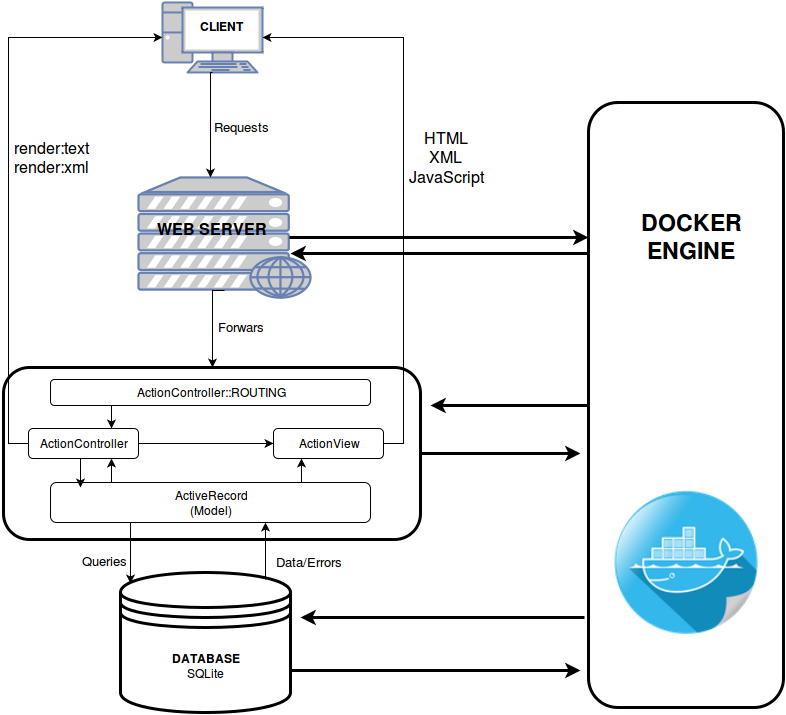
\includegraphics[width=\textwidth, height=\textheight, keepaspectratio]{component.png}}
  \caption{Component Architecturem}
  \label{fig:ca}
\end{figure}

\subsection{Initial Prototype}
\label{sec:prototype1}

Having the basic database structure, the team created some initial prototypes of the page, in order to discuss potential design changes. The first version of the page can be found in Figure 3.

\begin{figure}
  \centerline{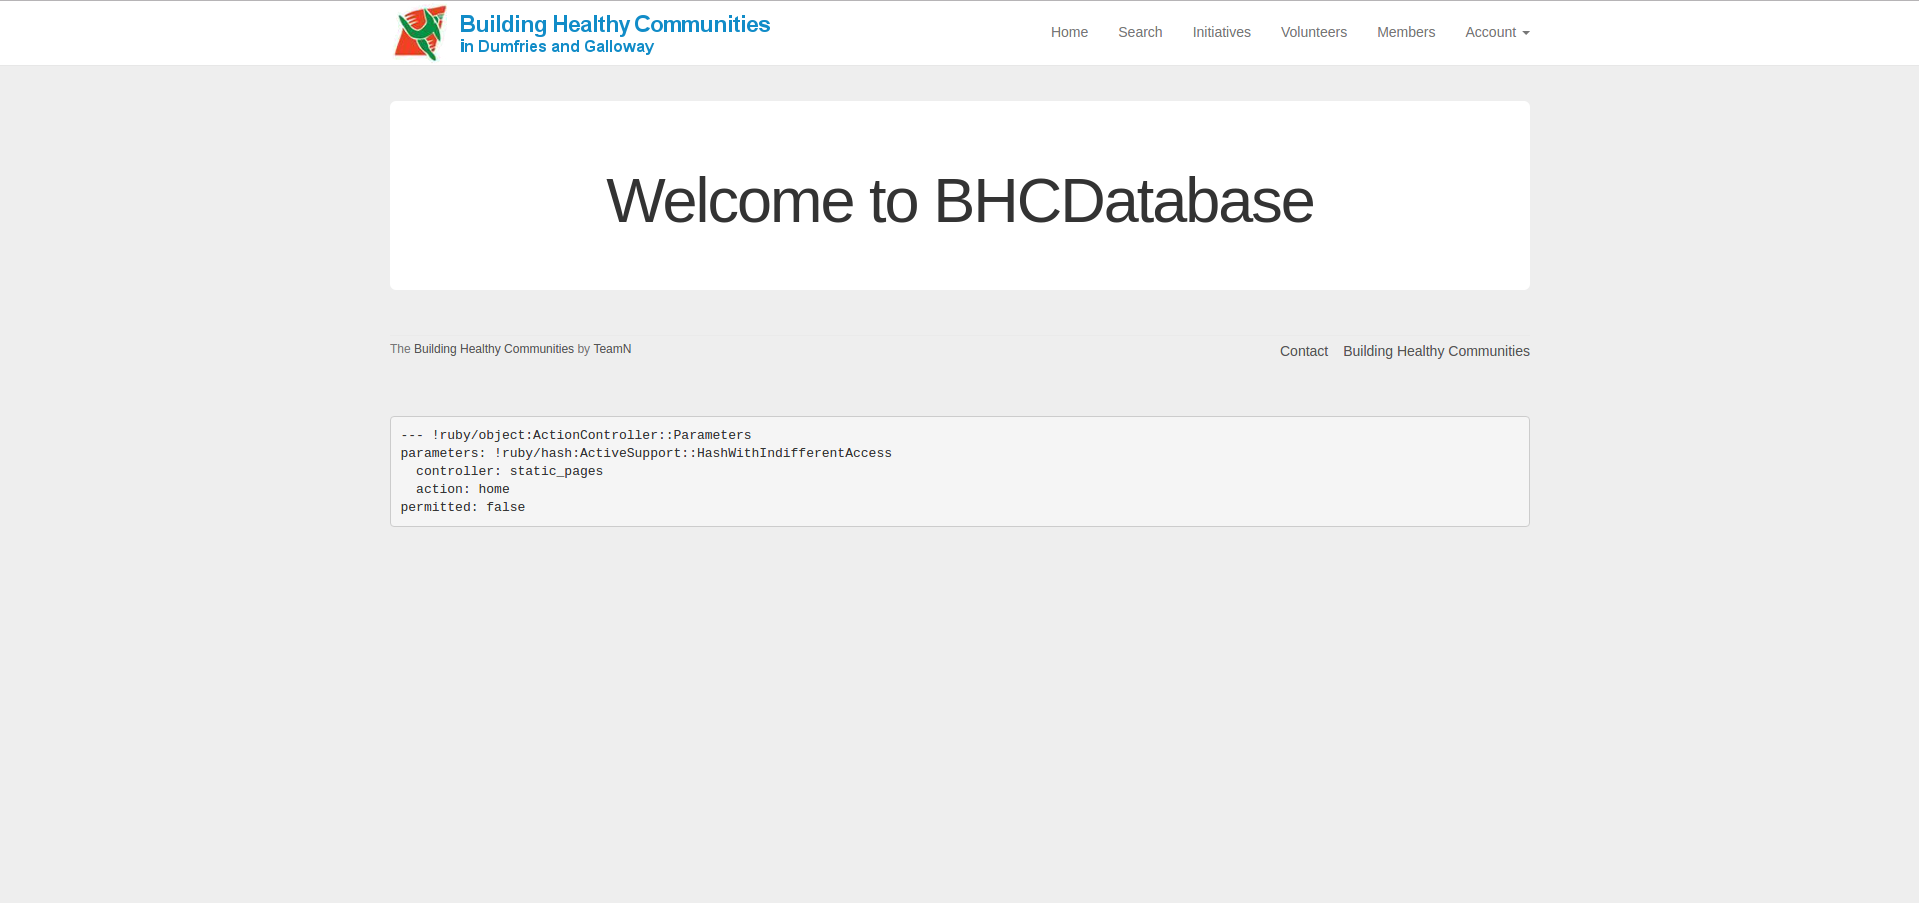
\includegraphics[width=\textwidth, height=\textheight, keepaspectratio]{oldhome.png}}
  \caption{Initial Prototype}
\end{figure}

The initial page is very basic, not very colourful and errors are contained. It was created to point out the idea of the  design and to outline a vision of how the site would work. The team decided to add the colours and the feel of the blog that the program already had.

\subsection{Final Prototype}
\label{sec:prototype2} 

The second design was more simplified in terms of account organisation. The customers clarified that the members would not be able to sign up, which has as a consequence to deleting this feature. Furthermore, the home page and the login page have been merged, so that a simpler view of the site is provided. The new prototype can be found in Figure 4.

\begin{figure}
  \centerline{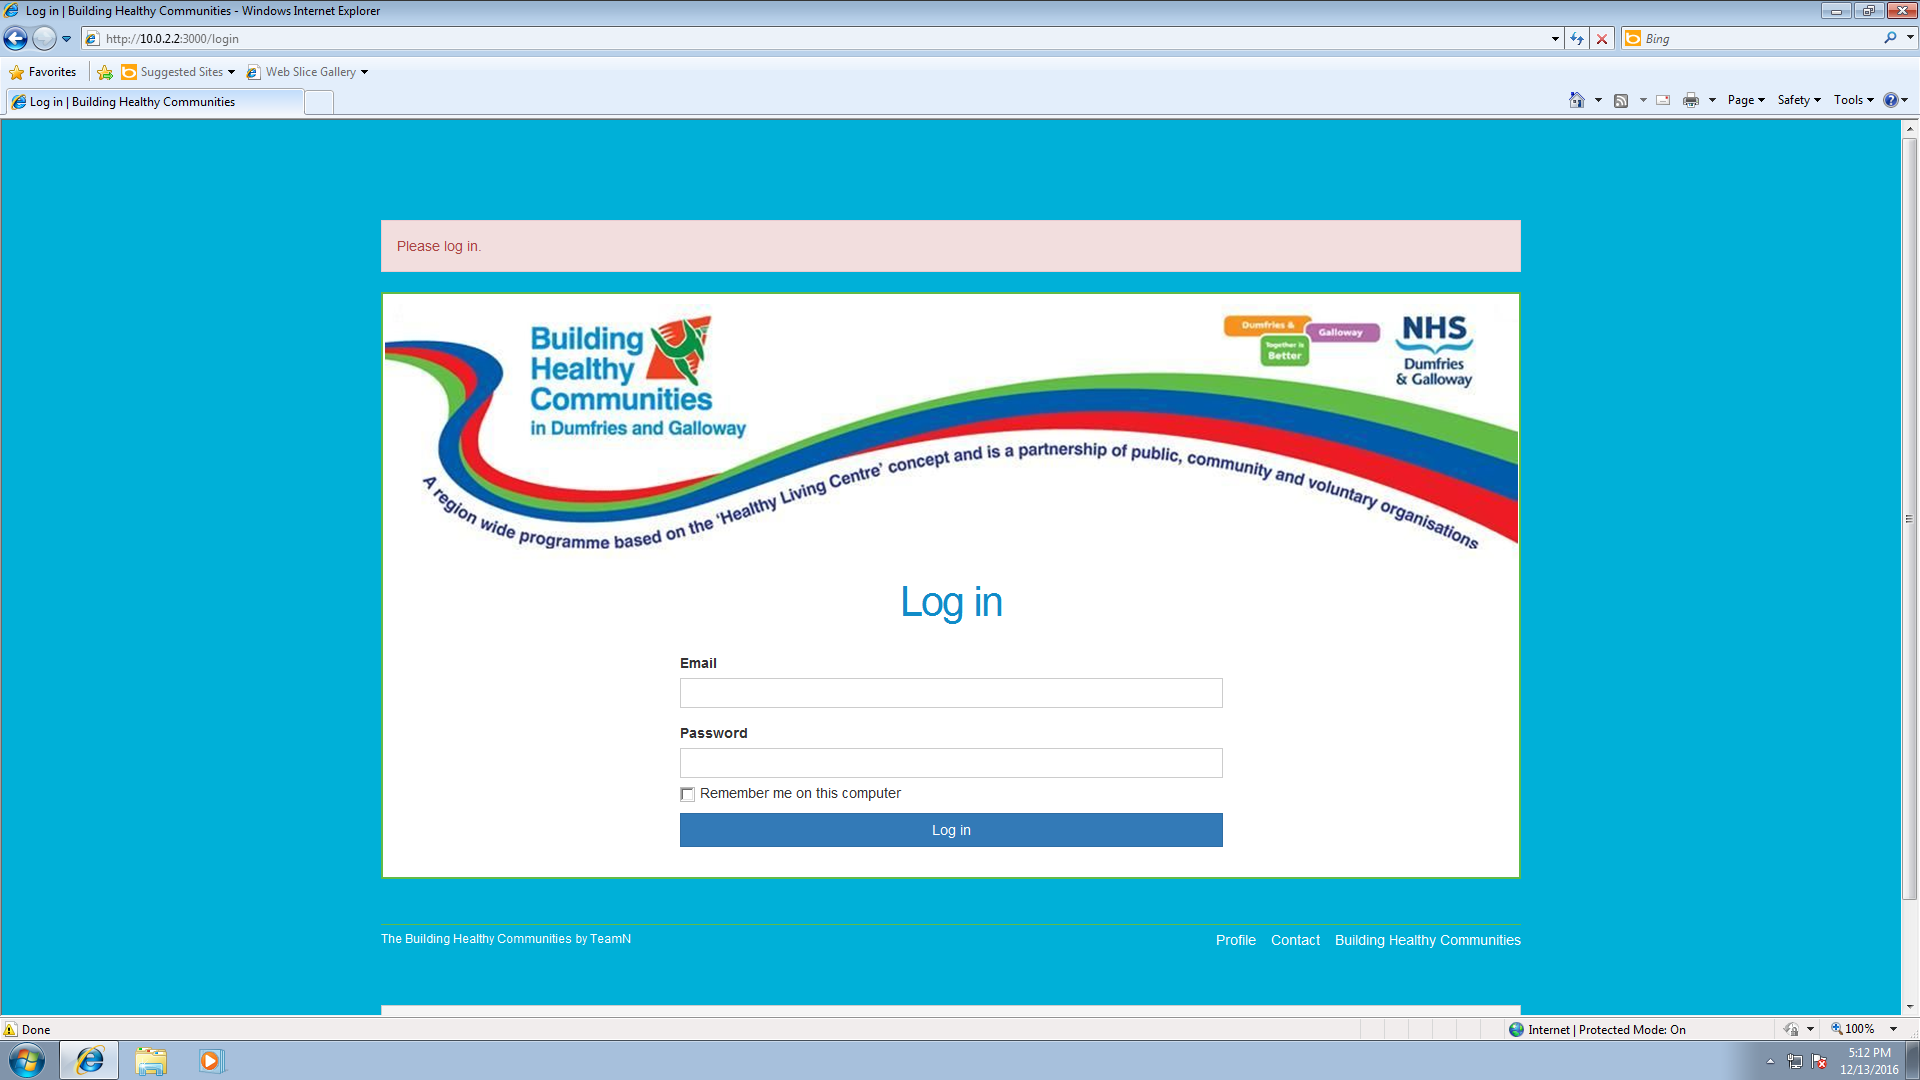
\includegraphics[width=\textwidth, height=\textheight, keepaspectratio]{newhome.png}}
  \caption{Second version of the prototype}
\end{figure}

 

\subsection{Component Diagram}
\label{sec:component}



\subsection{End of second and third milestone}
\label{sec:milestone23}

The above section was generally outlining the progress in the second and third milestone. The progress was steady and specific. By the 7th of December, the team had their third customer meeting was again used for further clarifications about the software implementation and navigation to some more complete wireframes. Furthermore, after the Christmas break and before the fourth customer meeting at the 26th of January, the team managed to create an initial version of the application. The application was presented to the customers on its current point and their opinion was asked. The customers were impressed with the amount of progress since in the previous customer meeting the back end development was not even started. Further clarifications were made about the navigation of the page, since know the customers had a visualisation of the application. Additionally, the customers requested a new feature which was never discussed before. The addition of a funding flag which represents which funding is from what organisation and where in which groups it is applied. Furthermore, different funding's apply to a specifying group of people and different funding's are applying to specified initiatives group.

The retrospective performed by the end of the second milestone, showed some lack of communication. The team did not consider this as a major issue since there was a three week holiday gap were everyone were focused on self studying about how to develop and deploy the application. Additionally, the team lacked on clarifying some basic features of the website with the customers. All the issues outlined on the second retrospective, they were clearly solved during the next. The team was more organised and communicative. Due to the fact that an initial stage of the application was presented on the fourth customer meeting lack of clarification of the features that was raised as an issue in the previous retrospective was know clearly solved.

%==============================================================================
\section{Working on the backend development}
\label{sec:backend}

\subsection{Objectives}
\label{objectives}

Before the beginning of the fourth milestone the team performed a meeting where the next objectives were outlined. Due to the fact that by the end of the current milestone the team should deliver a working version of the website the main focus was on resolving any opened issues that were raised from the previous retrospective and customer meeting. In the following weeks the website had all the added functionality created. The most critical issues that were raised is the newest demands that the customers were requested including the flag feature described above. The team had to discuss how this addition will be implemented.


\subsection{User Authentication}
\label{sec:authentication} 

Maybe the most important factor of the development of the site was the the protection of the user information.  A secure user authentication was a very crucial development part. By the phrase "User authentication" we mean the process where the user of the page types some credential information which are compared with the information that are kept in the database, if the information are matched the user is able to access various other information based on the level access that he/she has on the site. Improper development of the user authentication could lead to the leak of personal information from one user to another or the ability of every user editing the database. The team performed a small research online to explore the best practices of developing a highly secure user authentication. A highly suggested, "gem" for developing a good user authentication was the "Devise". Devise is one of the most popular user authentication tools. Some of its features are the ability of assigning multiple models in at the same time and its modulation. A user authentication tool such that provide a lot complexity and unnecessary tool that we will never user. On top of that, all these additional functionality may introduce issues that as programmers with a small experience may be unable to solve. All in all, a conclusion has been taken that a pre-built solution was not a very good idea. However, building from scratch the user authentication seemed a better solution since the complexity is controlled and every new feature is known along with any anomalies that may introduce. The user authentication was based in a very good book called "Ruby on Rails Tutorial (Rails 5)" written by Michael Hartl. The book provides some online tutorials which the authentication is based until chapter 6. The team finalised the authentication with some simple html commands based on previous experience.


\subsection{Browser and Mobile Compatibility}
\label{sec:compatibility} 

Our aim for browser compatibility is quite broad. From meetings with the customers, we have gathered the information that the support for the most popular browsers is essential, and that the website should function on iOS and Android (Running in both tablet and mobile form).

 A huge issue raised at that point, was the browser compatibility and more specifically the support of Internet Explorers version 7 and before. The earliest Internet Explorer version we aim to support is IE 8. This is because IE8 comes as standard with Windows 7. Although possible, we have chosen not to support IE 7 due to it coming with Windows Vista. Vista has 'Extended support until 11 April 2017.' After all, we have taken the decision not to support IE7, as to do so would be to support a soon to be dangerously out of date operating system. An important point to note is that Bootstrap only officially supports Internet Explorer 8-11.
 
 An important amount of the user's site, will only have as a mean of access to the site their mobile phones. Thus, a good mobile compatibility is demanded. Moreover, some screenshots have been taken from the initial prototypes of the page showing the mobile compatibility.

\begin{figure}
  \centerline{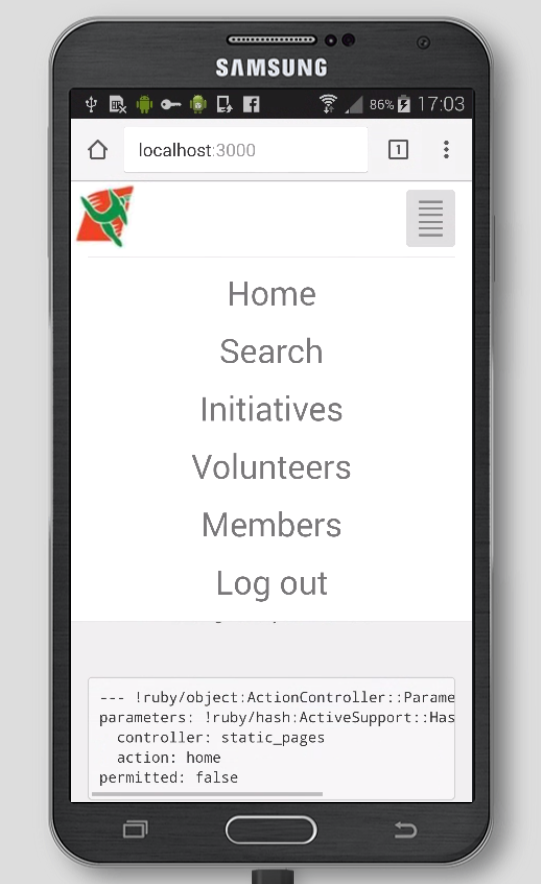
\includegraphics[ scale=0.3]{mobilePrototype.png}}
  \caption{Mobile Compatibility Prototype}
\end{figure}

\subsection{Testing}
\label{testing}

It is well known, that the development of any type of application is incomplete without the proper testings. Testing is a vital procedure in the process because it detects many defects and errors. Since the first day that we started coding, every section that we completed, we had also provided the proper testings. Providing testing in advance reduces the time and the cost needed to identify and correct defects. The graph provided in figure 6 displays the sharp increase of the costs of providing the defect tests very late in the process. The graph is from the level two "Software Engineering" course lecture notes.

\begin{figure}
  \centerline{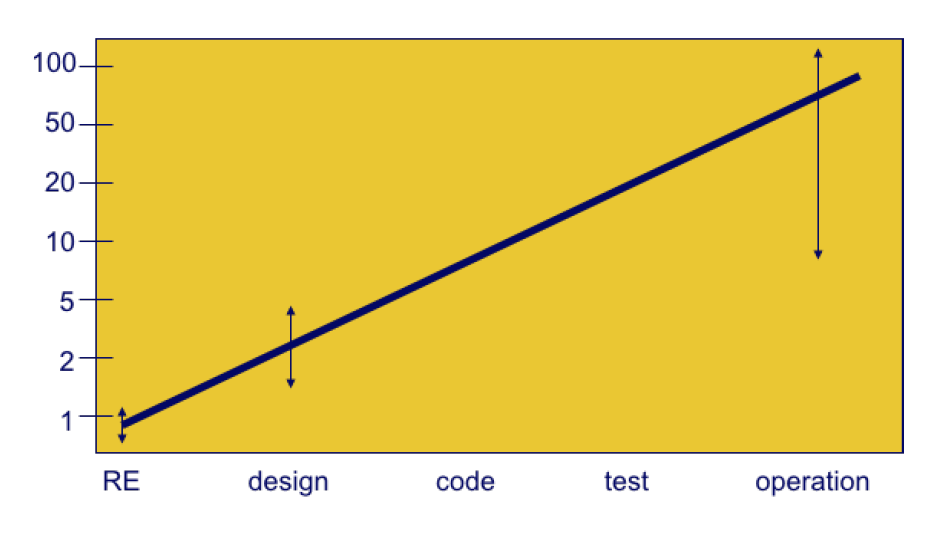
\includegraphics[width=\textwidth, height=\textheight, keepaspectratio]{costOfErrors.png}}
  \caption{Increasing rate of costs in different software development stages }
\end{figure}

 Gitlab's CI provides tests in every build using the \textit{.gitlab-ci.yml} file. Our file was using all the three stages provided: build, test and deploy. Then we have deployed the \textit{Runners}. A runner picks up a build in your project. Then, every time you commit or merge something in the repository, tests are running to check whether there are issues. Furthermore, the team developed their own tests using mutants. The program has an impressive percentage of testing coverage reaching more than 90\%. 
 
 
\subsection{Website Deployment}
\label{sec:deployment}

Having everything almost done and outline, the website is ready to be deployed and delivered to the customers.

\subsection{End of fourth milestone}
\label{sec:milestone4}

The fourth milestone was successfully completed with all its major goals succeeded. The website was successfully presented to its final stage to the customers on the customer meeting performed on the 23rd of February. Although some minor features were not yet implemented, a fully working version was delivered and in the following month all the features were progressively added. As usual, the team leader performed a navigation to the page and gave the customer's links were they could access the website. Unfortunately, the customers made more last minute demands to the team. This additions were added to the next milestone. The customers were asked to answer a questionnaire based on their navigation experience which was later used in the next milestone for the application evaluation.


%==============================================================================
\section{User Documentation}
\label{sec:user_doc}

One other important thing that we needed to create was the user documentation. Due to the fact that this is a university course, the software life cycle won't be strictly followed. For example, no future maintenance will take place. The team had to develop by the end of the development of the site a well defined user documentation. The documentation needed to be divided in two parts. The first part will be a brief documentation about how to navigate in the program and perform simple tasks such us adding a new user or deleting an old one. This was easily developed using a simple pdf file. A team member created a navigation document containing screenshots and arrows showing how to perform simple tasks in the website. Figure **number** contains a screenshot of the user manual.

\begin{figure}
  \centerline{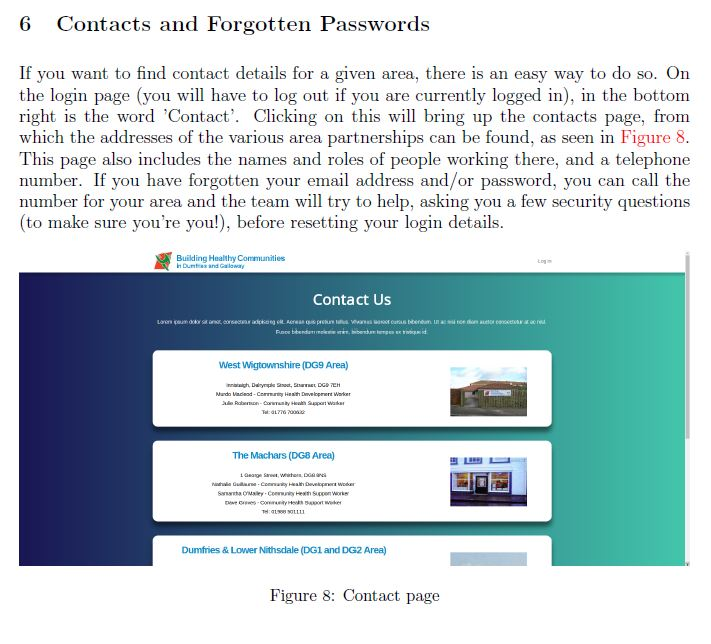
\includegraphics[width=\textwidth, height=\textheight, keepaspectratio]{usermanual.png}}
  \caption{User Manual }
\end{figure}

 The second part of the documentation is about explaining what technologies are used and generally how to manage the back-end development. Providing a well-understood documentation is highly important since the programs that are provided are funded. This results to the fact that they are economically depended to many different organisations that vary every year and these organisations vary the information that they need to be undertaken from the program users. The development of the documentation was based on a single rule, develop it such us every aspect, every word will be read by a small child. This way, the team managed to develop a well understood documentation. 

Having a written documentation as a separate file is not enough. The program, throughout the years will be used by many different people in many different places. The documentation will not be available to them all the time. As a consequence, the integration of a user guide in the page is essential. The team decided to use an already created engine called "how\_to". This engine enables both the user and the programmer to easily manage various documented sections of the website such us frequently asked questions and notifications explaining the usage of various fields.


%==============================================================================
\section{Formative Application Evaluation}
\label{sec:appEval}

A critical stage where maybe the most useful changes is the one of the Formative Application Evaluation. After the successful early deliver of the program to the customers, the team created a questionnaire and in combination with the simple user guide an application evaluation was performed. The evaluation was only performed from the customers. Due to the fact that the team had already discussed the design issues with the customers, the evaluation and questionnaire were mainly focused in the navigation and understanding of the page. On the  fourth customer day the team leader performed a navigation to the page, explaining to the customers how the page works.  Additionally, a user guide and a simple questionnaire was given. The goal was for the team to study whether the customers are able to navigate to the page and if they are able to solve their issues through the usage of the user guide. For the creation of the questionnaire a simple "Google Form" was used. The questionnaires were collected and studied. The questionnaire can be found in Figure ***number***.

\begin{figure}
  \centerline{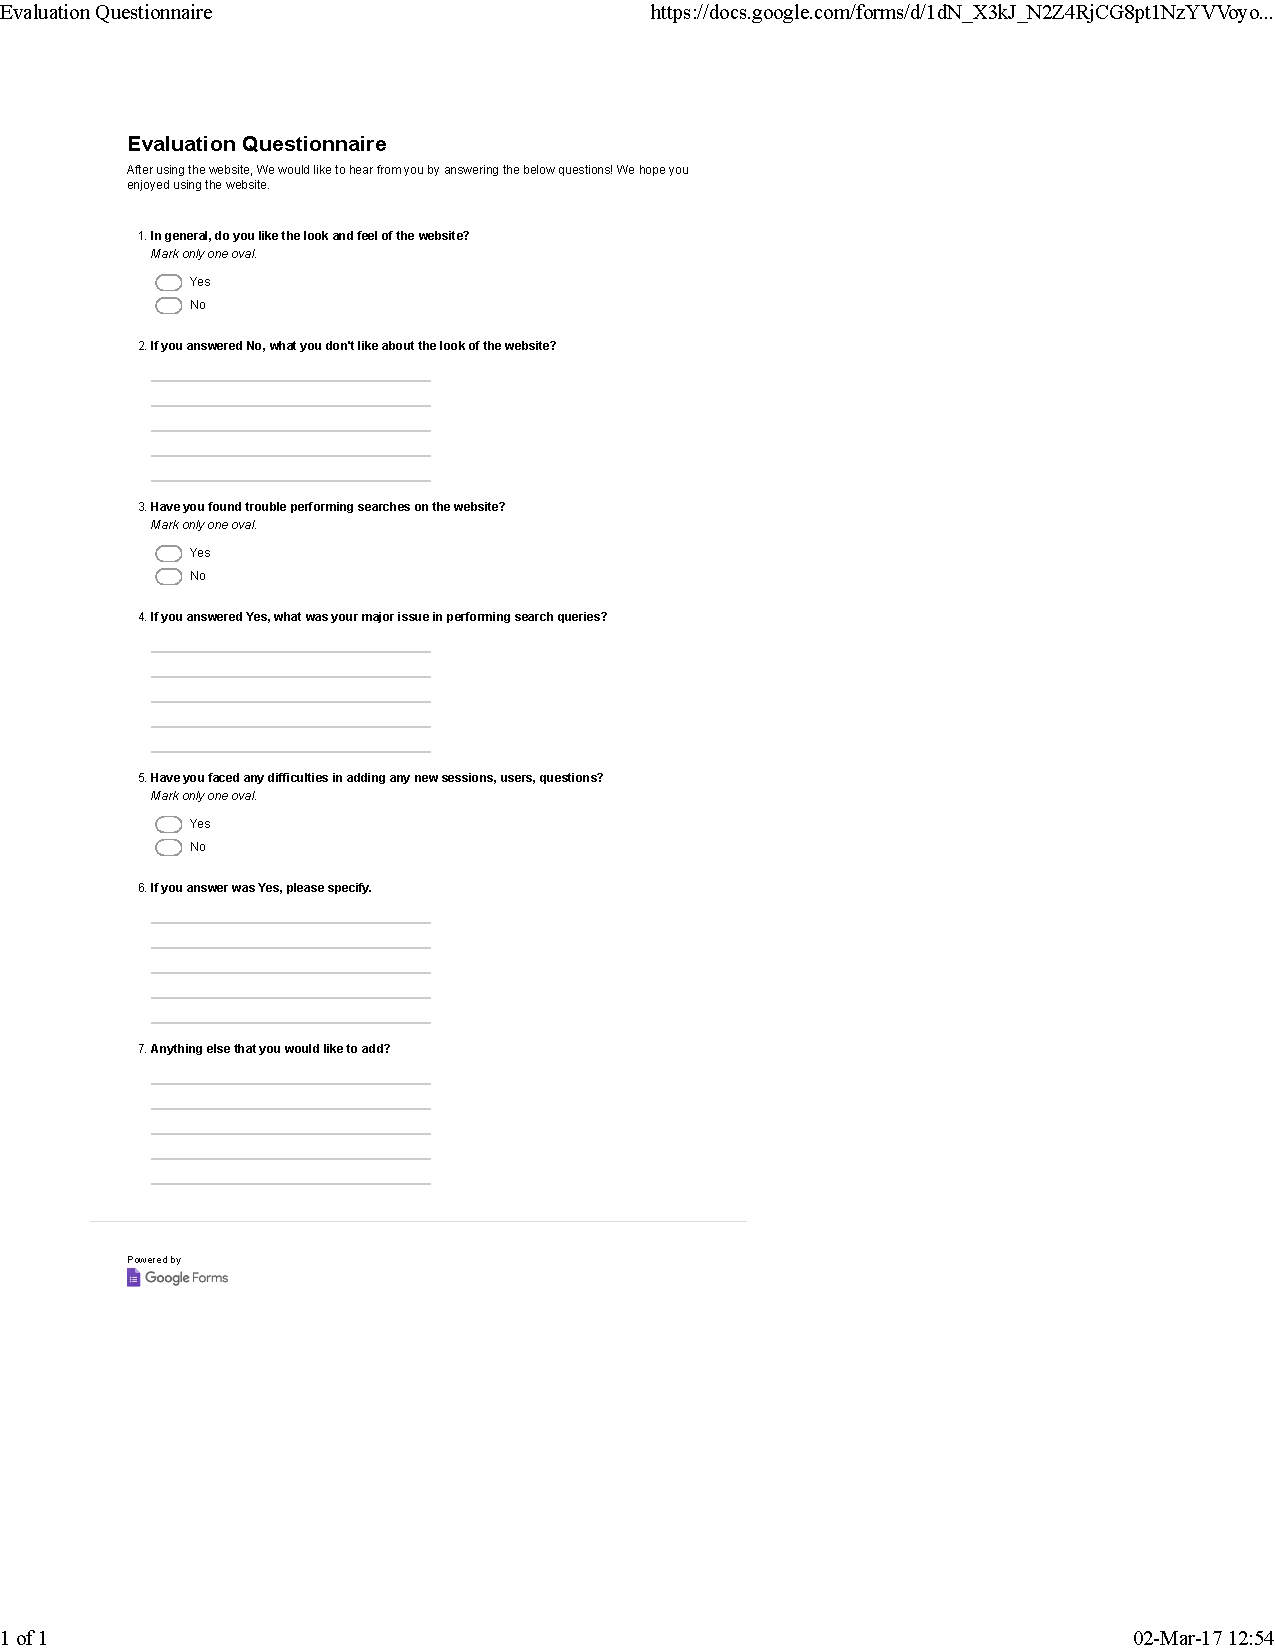
\includegraphics[width=\textwidth, height=\textheight, keepaspectratio]{evalQuestCustomers.pdf}}
  \caption{Evaluation Questionnaire for customers }
\end{figure}

As a consequence of having a small amount of responses the results where mainly qualitative than quantitative. The responses of the questionnaire showed no major issues except of the fact that they have asked more features that again were not discussed in previous meetings. The team focused on solving the small navigation issues that the customers identified and left the new features in the case of having some more time.





%==============================================================================

\section{Challenges}
\label{challenges}

Developing a site from scratch, always creates some major challenges. The second and third retrospective were pretty representative for stating what challenges the team faced and some suggestions of how they were solved. Usually a team has a major issue developing test. Tests were mainly time consuming since we needed enormous amounts of tests. Surprisingly, the tests had a very high coverage of an approximate 90% .

The organisation of the database was another big challenge that the team have encountered. Although the database was characterised by its simplicity, retrieving the information was tricky since a member of a team could be a volunteer in another team and a general admin. This raised some authentication issues whether where that specific user is allowed to alternate information and where is not.

As in every project developing process, programmers will face some last-minute demands from the customers. One of these demands were the creation of some type of flag pointing which members or groups are funded from specific organisations. The current demand raised some issues in in the database development since this is an addition very specific information regarding every member of every group. The team assigned that as an extra feature which would be developed if there was time, something that was stated clear from the very first day that it was suggested. The feature caused last minute additions to the ER diagram. The team managed to create the feature and successfully add it to the site.

Since we are Agile team, we had another change of the initial requirements regarding the deadline for delivering the final product - we were asked to be ready one month before the due date. In that way the customers would have a month to test the application and to give us feedback.This was quite a challenge for the team because there still was a lot of work to be done. The team managed to deliver the software on time but without same minor features which were progressively added in the software.

Another thing the team was asked to do, as previously mentioned, was the User Manual. This documentation would be useful for the current customers and for any other future users of the application. In that way they can have a simple and brief guidance how to navigate through the application and to take as much advantage of it as they could.



%------------------------------------------------------------------------------
\section{Final Customer Day}
\label{sec:finalDay}





%------------------------------------------------------------------------------

% - - - - - - - - - - - - - - - - - - - - - - - - - - - - - - - - - - - - - - -
\section{Knots and Bundles}
\label{sec:managing}


%------------------------------------------------------------------------------
\section{Conclusions}

Taking everything into account, designing and developing a software application wasn't an easy process. Considering the fact that the team was consisted of six novice students with no experience at all at agile software programming, the resulting presented material was more than satisfactory. Having real customers with high demands was definitely a challenge. By the adaptation of several techniques and methodologies every difficulty was successfully confronted.

Agile programming proved it self that is a very good practice to be followed from novice students. Pair programming played a critical role in terms of identifying bugs and errors in the code. By the early weeks the team lacked of organisation but the team reviewed some valuable Agile programming rules and with some team reorganisation valuable time was definitively saved. Communication was also identified to be extremely important, since many major issues that could not be solve from one, were solved from another. Although, at some point during the Christmas's break the team faced some communication issues, they were not considered important since the team was already in a very good position in the project so very few things were done during the break. Christmas break was mainly dedicated on revising and self studying about the project. Putting in practice so many technologies such as Ruby and Docker was undoubtedly one of the hardest task that the team had to undergo. Thus, during the Christmas break a wiki page was created which pointed out many useful sites for self-studying and self-practicing.

One of the best practices that were kept, was to strictly follow the university guidance and create test cases for each new aspect we created in the application. The test cases identified many bugs and errors which the team managed to successfully solve. Many other teams did not kept that practice and as a result many serious issues were not identified in advance resulting to the inability of delivering their software within the time constraints.

Furthermore, branching was another important practice that we kept. The team followed a strict plan of creating a new branch for every issue and resolving that issue in the branch. After everything are checked and tested, a merge request is created which only two of the six team members can accept after inspecting the code for conflicts. Thus, the master branch was always in a fully working condition with the testing percentage to be from the very beginning at 80-90$%$. Performing frequent commits also helped the testing to be constantly kept high.

Delivering a software do not only demand to create a code but to create a software exactly the same with the customers visions, realistically of course. Despite the fact that the clients where characterised by politeness and cooperation, they were very high demanding. Until the very last week new features were requested. After endless hours of re-factoring the system the team managed to deliver as many features as they were able. The team learned that even with such demanding clients, you have to always tell the truth to the clients. When the team decides that due to time constraints a feature cannot be implemented or even when the team does not know how to implement a feature, the customers must be contacted and the issue must be discussed. Promising features that will never been delivered will result to a mistrustful relationship between the clients and the developing team. This experiences helped the team to realise that requirements negotiation is an important factor in the software development process.

On the 24th of February the team managed to deliver a fully working website to the customers. Furthermore, on the 22 of March, final demonstration date, an improved website with added functionality was delivered to its final state.

To conclude, working with real clients, gave to each member the opportunity to develop a minor working experience, to realise how the future is going to be and develop the proper bases needed for working in a real company. Every student discovered in more depth their abilities and weakness and most importantly learned that a customer has not only a vision but also important requirements that need to be followed step by step. Everyone managed to develop professionalism were you have to constantly communicate with inexperienced customers and listen with respect their demands, even when they are impossible to be developed. Backtracking the experience, everyone managed to develop new skill that will be later used in their software engineering career. 

%==============================================================================
\bibliographystyle{plain}
\bibliography{dissertation}
\subsection{Bibliography}
\label{Bibliography}


\label{tech}
Technology
\begin{itemize}

\item "wikipedia.org: Ruby on Rails"
\newline https://en.wikipedia.org/wiki/Ruby\_on\_Rails[Accessed 14 December 2016]

\item "wikipedia.org: Django"
\newline https://en.wikipedia.org/wiki/Django\_(web\_framework) [Accessed 14 December 2016]

\item "skilledup.com: Comparison of Django and Rails
\newline http://www.skilledup.com/articles/battle-frameworks-django-vs-rails [Accessed 14 December 2016]

\item "wikipedia.org: RubyGems"
\newline https://en.wikipedia.org/wiki/RubyGems [Accessed 14 December 2016]

\item "postgresql.org: PostgreSQL"
\newline https://www.postgresql.org/ [Accessed 14 December 2016]

\item "docker.com: What is Docker?"
\newline https://www.docker.com/what-docker [Accessed 26 January 2017]


\end{itemize}




\label{user_stories}

User stories

\begin{itemize}

\item "agilemodeling.com:User stories"
\newline http://www.agilemodeling.com/artifacts/userStory.html [Accessed 26 December 2016]

\end{itemize}


\label{er}
Entity Relationship diagram

\begin{itemize}

\item "smartdraw.com: ER diagram"
\newline https://www.smartdraw.com/entity-relationship-diagram/ [Accessed 12 January 2017]

\end{itemize}

\label{authentication}
User authentication

\begin{itemize}

\item " searchsecurity.techtarget.com: User authentication"
\newline http://searchsecurity.techtarget.com/definition/authentication [Accessed 15 January 2017]

\item "github.com: Devise"
\newline https://github.com/plataformatec/devise [Accessed 15 January 2017]

\item "railstutorial.org: Ruby on Rails Tutorial (Rails 5) By Michael Hartl"
\newline https://www.railstutorial.org/book/ [Accessed 15 January 2017]

\end{itemize}

\label{testing}

Testing

\begin{itemize}

\item "docs.gitlab.com: Continuous Integration (CI)" 
\newline https://docs.gitlab.com/ce/ci/quick\_start/README.html [Accessed 19 January 2017]

\end{itemize}

\label{authentication}

User Authentication
\begin{itemize}

\item "github.com: How\_to user documentation"
\newline https://github.com/amuntasim/how\_to


\end{itemize}





\end{document}
